\documentclass[a4paper,10pt]{article}
\usepackage[utf8]{inputenc}
\usepackage{graphicx}


%opening
\title{Recipe book}
\author{}

\begin{document}

\maketitle
\section{Brownies}
Line baking dish with parchment paper.
\begin{itemize}
 \item Unsalted butter 225 grams
 \item Eggs 3
 \item Coffee tablespoon
 \item Salt 1/8th teaspoon
 \item Vanilla extract 1 tea spoon
 \item Granulated sugar 200 grams
 \item Brown sugar 200 grams
 \item Flour 120 grams
 \item Cocoa powder 120 grams
 \item chopped chocolate 200 grams
\end{itemize}

\vspace{0.5cm}

\noindent Melt butter and chocolate while stirring. Add cocoa powder while warm and whisk. Add in sugars, then eggs. Finally salt and vanilla extract. Fold in flour. Bake at 180 for 28 minutes for 2-3 cm thick layer.

\newpage


\section{Chocolate chip cookies}
Source: through Bastian Havers, original:Timothy (Basti's colleague?)

Ingredients:
\begin{enumerate}
 \item 380g all purpose wheat flour
\item 1tsp baking soda
\item 1 tsp salt (you can skip this if
you use salted butter if you
want)
\item 225g butter (soft at room
temperature)
\item 80g white sugar or raw
crystalized sugar
\item 270g brown sugar
\item 2tsp vanilla extract
\item 1-2 eggs (one is usually
enough, but sometimes I do
two)
\item 340g rough chopped
chocolate
\end{enumerate}

Steps:
In a bowl, mix the flour, baking
soda, and salt.
In a large bowl, mix the sugars
and butter until creamy. Stir in
the vanilla.
Stir together the dry ingredients
into the sugar-butter mix until
partially blended. Stir in the eggs.
Add the chocolate (it can be
helpful to work in batches with
the chocolate, to distribute it
evenly). Mix together thoroughly
with a spoon, spatula, or hands.
Once the dough is mixed, you can
bake immediately (but if the
dough feels loose, it's useful to
chill it for a while first). But I
recommend that you form the
dough into a large ball, cover it in
paper or plastic wrap, and leave it
to marinate in the refrigerator for
at least 24 hours (but not more
than 72 hours). This is where the
flavor and texture develops. The
longer you leave it, the tighter
the dough will be, and it will
make thicker cookies. The
shorter, the looser the dough and
flatter the cookies. The longer
you leave it, the more the dough
will take on a butterscotch flavor.
Generally, I prefer dough that's
been in the fridge for 48-72
hours, since I think the flavors
mature a bit, and the texture of
the cookie is nicely balanced
between soft and firm.
When ready to bake, preheat the
oven to 175. Take the dough from
the fridge and let it get close to
room temperature before baking.
Use baking paper on a metal
sheet tray. Scoop the cookie
dough in ball-shaped dollops. I
usually aim for about 2tbsp
scoops, but this is partly a matter
of preference.
Bake for 12-13 minutes for
cookies that stay soft after
cooling. Bake for 15 or a little
longer for crispier cookies.
Let them cook and firm up a bit
after baking.
Notes:
For the chocolate, I usually prefer
something with a high cocoa
percentage (70\% or higher; I
really like using 90\%). The cookies
are sweet enough from the sugar,
and the bitterness balances it out.
Chopping chocolate is a matter of
preference: make them as coarse
or fine as you want. You could
use premade chips as well.
You have a lot of options with the
sugars to get to different flavors.
The sugar should be
approximately 90-95\% of the
weight of the flour. I've played
around with different blends of
sugars, but the balance in the
ingredient list is my staple.
\newpage
\section{Artichoke dip}
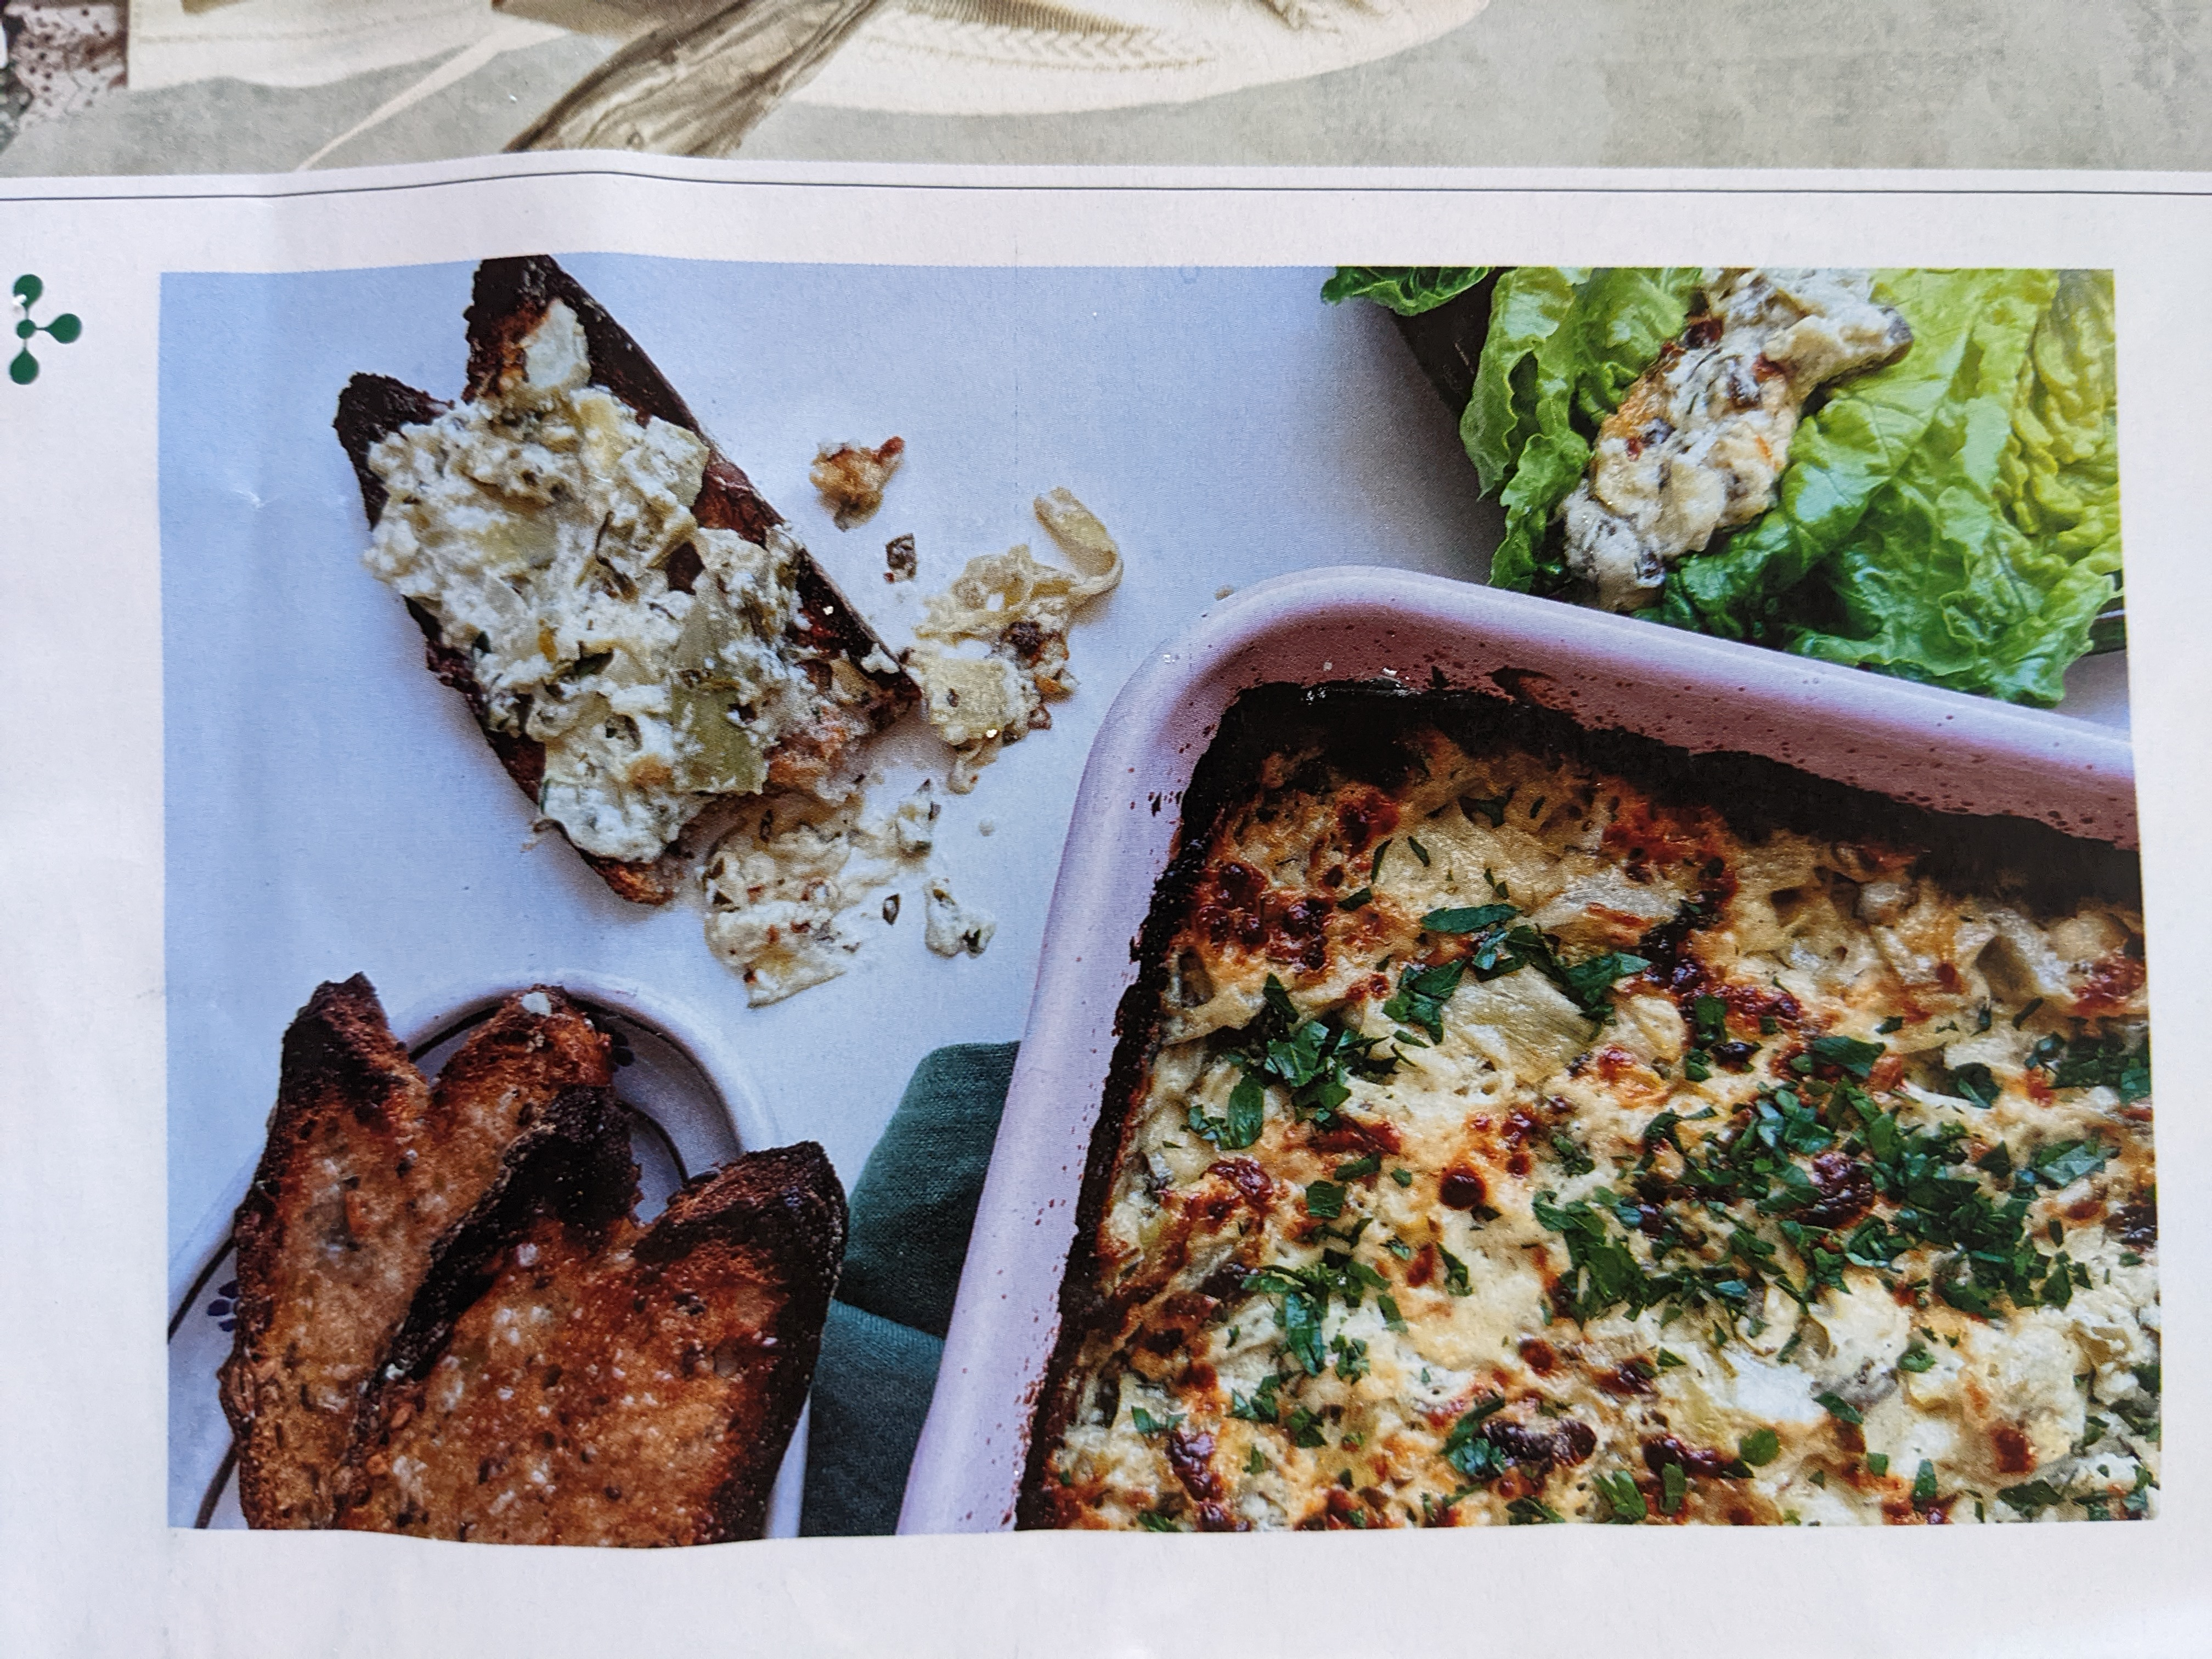
\includegraphics[scale=0.07,angle=90]{./images/artichoke_dip_1.jpg}
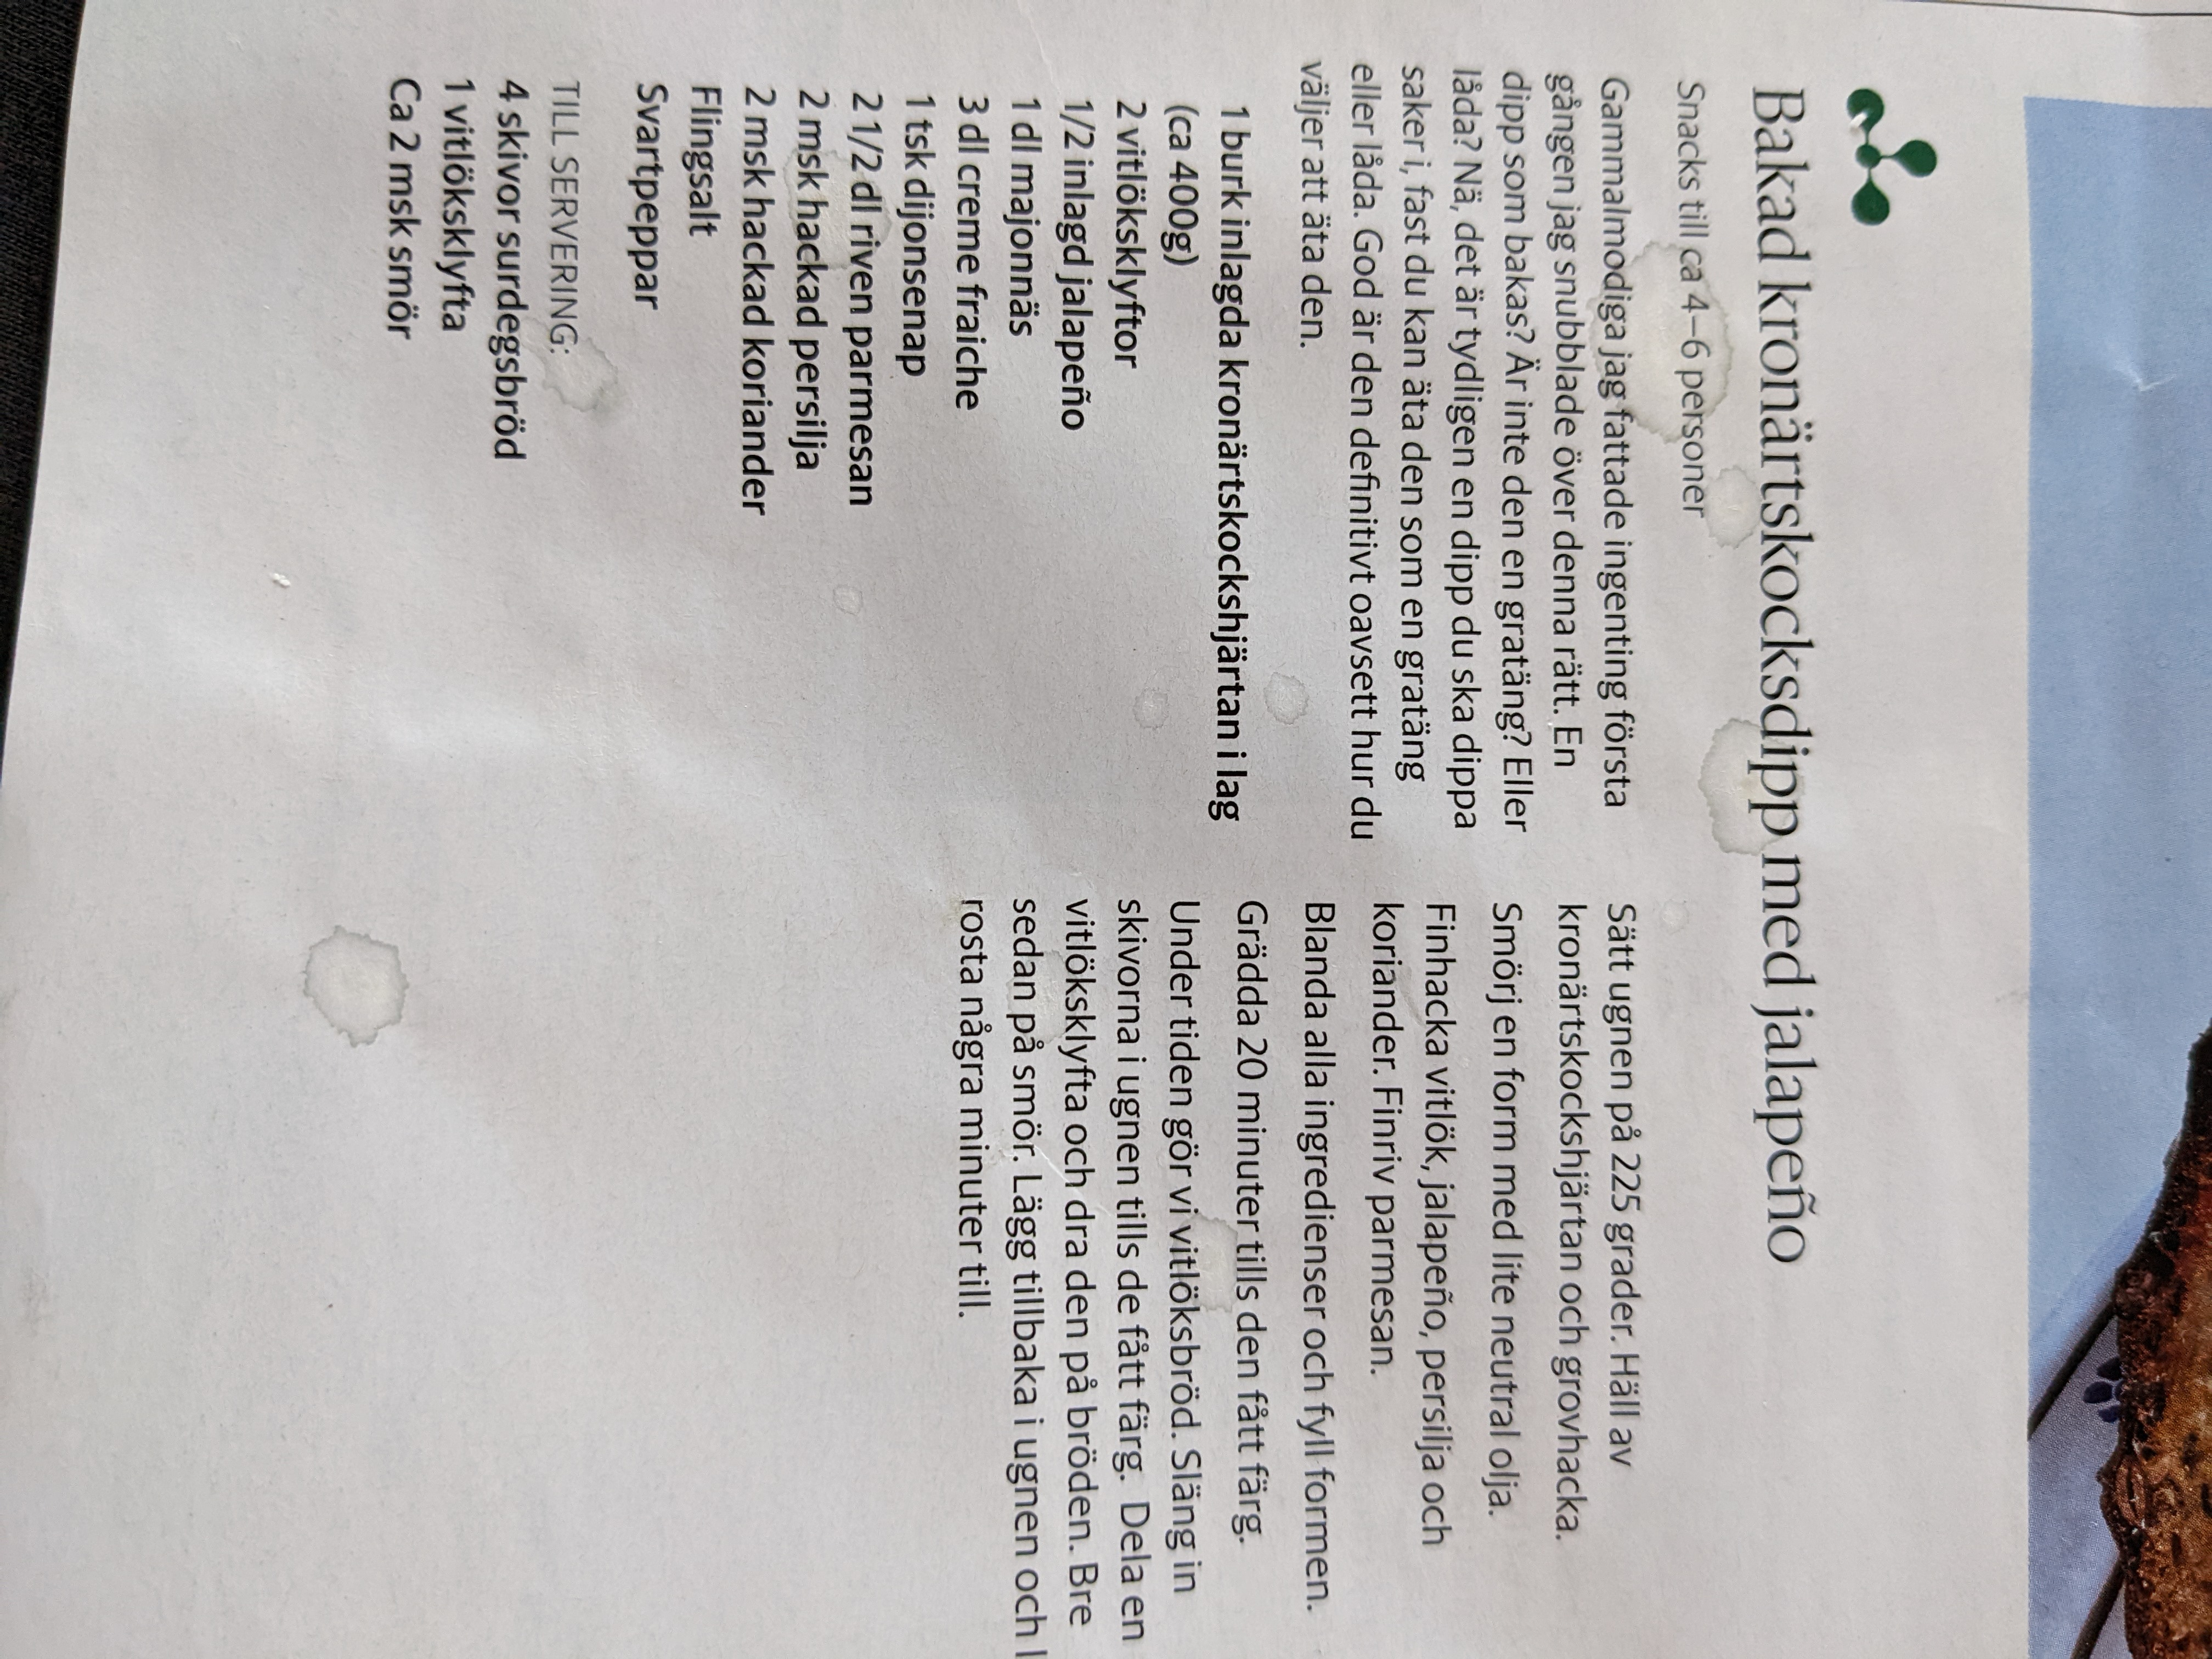
\includegraphics[scale=0.07,angle=90]{./images/artichoke_dip_2.jpg}
\newpage

\section{Tzatziki}

\newpage
\section{Pumpkin chickpea curry}

\end{document}
    
